\documentclass{article}
\usepackage[%
    left=0.5in,%
    right=0.5in,%
    top=0.5in,%
    bottom=0.5in,%
]{geometry}%
\usepackage{minitoc}
\usepackage{multicol}
\usepackage{graphicx}
\usepackage{fixltx2e}
\usepackage{hyperref}
\usepackage{hyperref}
    \hypersetup{ colorlinks = true, linkcolor = blue }
\usepackage{blindtext}

\graphicspath{ {./} }

\newcommand{\inlinecode}[2]{\colorbox{lightgray}{\lstinline
[language=#1]$#2$}}
\newcommand{\worddef}[1]{\hyperref[sec:reference]{\textit{#1}}}

\begin{document}

\section{Virtual memory}
\begin{flushleft}
\textit{Translation look aside buffers} (\textbf{TLBs}) are (usually) located inside the \textit{memory management unit}.
\begin{itemize}
	\item They \textit{cache} the \textbf{most frequently used} page table entries
	\item They can be searched in \textbf{parallel}
	\item The principle behind TLBs is similar to other types of \textbf{caching} in operating systems
	\item \textbf{Remember}: locality states that processes make a large number of references to a small number of pages
\end{itemize}
\end{flushleft}

\section{Page tables}
\begin{flushleft}
A \textbf{“normal”} page table’s size is proportional to the \textbf{number of pages} in the virtual address space, this can be prohibitive for modern machines.\\
An \textbf{“inverted”} page table’s size is proportional to the size of \textbf{main memory} (RAM)
\begin{itemize}
	\item The inverted table contains \textbf{one} entry for every \textbf{frame} (i.e. not for every page), and it indexes entries by \textbf{frame number}, not by page number.
	\item When a process references a page, the OS must search the (\textbf{entire}) \textit{inverted page} table for the corresponding entry (i.e. page and process id), this could be too slow.
	\item Solution: Use a \textit{hash function} that \textbf{transforms} page numbers (n bits) into frame numbers (m bits) - Remember: $n > m$.
\end{itemize}
\end{flushleft}

\subsection{Inverted page tables}
\begin{itemize}
	\item The frame number will be the index of the inverted page table.
	\item \textbf{Process Identifier} (PID) - The process that owns this page.
	\item \textbf{Virtual Page Number} (VPN)
	\item \textbf{Protection bits} (Read/Write/Execution)
	\item \textbf{Chaining Pointer} - This field points toward the next frame that has exactly \textbf{the same VPN}. We need this to \textbf{solve collisions}.
\end{itemize}
\begin{center}
	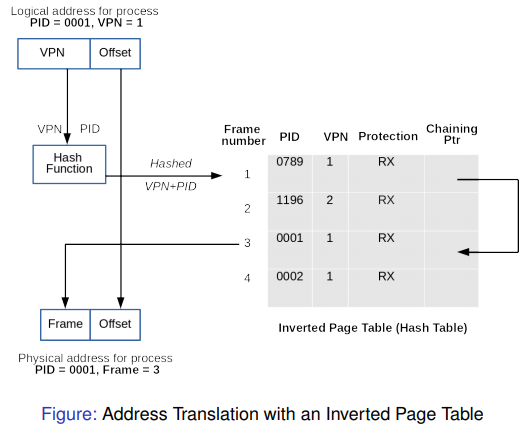
\includegraphics[scale=0.6]{inverted_table.png}
\end{center}

\bigskip
\begin{flushleft}
\textbf{Advantages}:
\begin{itemize}
	\item The OS maintains a \textbf{single} inverted page table for all processes
	\item It \textbf{saves} lots of space(especially when the virtual address space is much larger than the physical memory) 
\end{itemize}
\textbf{Disadvantages}:
\begin{itemize}
	\item Virtual-to-physical translation becomes much \textbf{harder/slower}.
	\item Hash tables eliminates the need of searching the whole inverted table, but we have to \textbf{handle collisions} (that will also slow down the translation).
\end{itemize}
TLBs are \textbf{particularly necessary} to improve their performance.
\end{flushleft}

\subsection{Page loading and replacing}
\begin{flushleft}
Two key decisions have to be made using virtual memory.
\begin{itemize}
	\item What pages are \textbf{loaded} and when \verb!->! predictions can be made
	\item What pages are \textbf{removed} from memory and when \verb!->! page replacement algorithms 
\end{itemize}
Pages are \textbf{shuttled} between primary and secondary memory
\end{flushleft}

\subsection{(On)demand paging}
\begin{flushleft}
\textit{Demand paging} \textbf{starts} the process with \textbf{no pages} in memory:
\begin{itemize}
	\item The first instruction will immediately cause a \textit{page fault}
	\item More page faults will follow, but they will \textbf{stabilise} over time until moving to the next \textit{locality}.
	\item The set of pages that is currently being used is called its \textit{working set} (resident set)
	\item Pages are only loaded \textbf{when needed}, i.e. following \textit{page faults}
\end{itemize}
\end{flushleft}

\subsection{Predictive paging}
\begin{flushleft}
When the process is started, \textbf{all pages} expected to be used (i.e. the working set) could be brought into memory \textbf{at once}.
\begin{itemize}
	\item This can drastically \textbf{reduce} the page fault rate
	\item Retrieving multiple (contiguously stored) pages \textbf{reduces} transfer times (seek time, rotational latency, etc.) 
	\item Pre-paging loads pages (\textbf{as much as possible}) before page faults are generated (a similar mechanism is used when processes are swapped out/in)
\end{itemize}
\end{flushleft}

\subsection{Implementation details}
\begin{flushleft}
Avoiding unnecessary pages and page replacement is important!. Let m$a, p$ and $pft$ denote \textbf{the memory access time} (2 times for single-level page tables) (ranging from 10 to 200ns), page fault rate, and page fault time, respectively, the effective access time is then given by:
\[ T_{a} = (1 - p) * ma+pft * p \]
Note that we are \textbf{not} considering \textbf{TLBs} here.\\
The \textbf{expected/effective} access time is \textbf{proportional} to \textit{page fault} rate when keeping page faults into account. \textbf{Ideally}, all pages would have to be loaded \textbf{without} demand paging
\end{flushleft}

\section{Page replacement}
\subsection{Concepts}
\begin{flushleft}
The OS must choose a page to \textbf{remove} when a new one is loaded (and all are occupied). This choice is made by \textbf{page replacement algorithms} and takes into account:
\begin{itemize}
	\item When the page is last \textbf{used/expected} to be used again
	\item Whether the page \textbf{has been modified} (only modified pages need to be written)
	\item Replacement choices have to be made \textbf{intelligently} (random) to save time/avoid thrashing
\end{itemize}
\textbf{Alogrithms}:
\begin{itemize}
	\item \textbf{Optimal} page replacement \\
	When a page needs to be swapped in, the operating system swaps out the page \textbf{whose next} use will occur farthest in the future. For example, a page that is not going to be used for the next 6 seconds will be swapped out over a page that is going to be used within the next 0.4 seconds. It \textbf{cannot} be implemented in general OS.

	\item \textbf{FIFO} page replacement\\
	The \textbf{simplest} low-overhead page-replacing algorithm that requires little bookkeeping on the part of the operating system. The OS \textbf{keeps track} of all the pages in memory in a queue, with the \textbf{most recent} arrival at the back, and the oldest arrival in front. When a page needs to be replaced, the page \textbf{at the front} of the queue (the oldest page) is selected. While FIFO is cheap and intuitive, it performs \textbf{poorly} in practical application

	\item \textbf{Second chance}\\
	A modified form of the FIFO, works by looking \textbf{at the front} of the queue. It checks to see if its \textbf{referenced} bit is set. If it is not set, the page is \textbf{swapped out}. Otherwise, the referenced bit is \textbf{cleared}, the page is inserted \textbf{at the back} of the queue (as if it were a new page) and this process is repeated.
	
	\item \textbf{Clock replacement}
	Performs the same general function as Second-Chance. Keeps a circular list of pages in memory, with the "hand" (\textbf{iterator}) pointing to the last examined page frame in the list. When a page fault occurs and no empty frames exist, then the R (\textbf{referenced}) bit is inspected at the \textbf{hand's} location. If R is \texttt{0}, the new page is put in place of the page the "hand" points to. Otherwise, the R bit is cleared, then the clock hand is incremented and the process is repeated until a page is replaced.
	
	
	\item Not recently used (\textbf{NRU}) \\
	Favours \textbf{keeping pages} in memory that have been \textbf{recently} used. This algorithm works on the following principle: when a page is referenced, a referenced bit is set for that page, marking it as referenced. Similarly, when a page is modified (written to), a modified bit is set. At a certain fixed time interval, a timer \textbf{interrupt triggers} and \textbf{clears} the referenced bit of all the pages, so only pages referenced within the current timer interval are marked with a referenced bit. 

	\item Least recently used (\textbf{LRU})
	Works on the idea that pages that have been \textbf{most heavily used} in the past few instructions are most \textbf{likely} to be used heavily in the next few instructions too. While LRU can provide \textbf{near-optimal} performance in theory (almost as good as adaptive replacement cache), it is \textbf{rather expensive} to implement in practice. 
\end{itemize}
\end{flushleft}

\pagebreak
\section*{Reference section} \label{sec:reference}
\begin{description}
	\item[placeholder] \hfill \\
\end{description}
\end{document}
